\documentclass{standalone}
\usepackage{tikz,amsmath}
\begin{document}
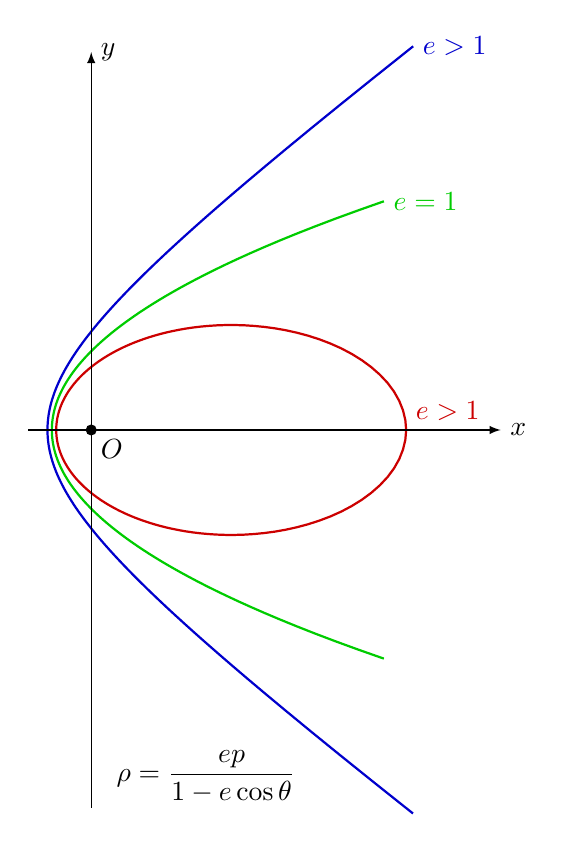
\begin{tikzpicture}[>=latex, scale=2]
  \draw [domain=0:360,samples=200,thick,red!80!black] plot (\x:{0.4/(1-0.8*cos(\x))});
  \draw [domain=38:322,samples=200,thick,green!80!black] plot (\x:{0.5/(1-cos(\x))});
  \draw [domain=50:310,samples=200,thick,blue!80!black] plot (\x:{0.625/(1-1.25*cos(\x))});
  \draw[->] (-0.4,0)--(2.6,0)node[right]{$x$};
  \draw[->] (0,-2.4)--(0,2.4)node[right]{$y$};
  \node at (38:2.359)[right,green!80!black] {$e=1$};
  \node at (50:3.180)[right,blue!80!black] {$e>1$};
  \node at (2,0)[above right,red!80!black] {$e>1$};
  \node at (0.1,-2.2)[right] {$\rho=\dfrac{ep}{1-e\cos\theta}$};
  \fill (0,0)circle(1pt)node [below right]{$O$};
  \end{tikzpicture}
\end{document}